%\documentclass[slides]{beamer} %switch "slides" to "handout" for printing out
\documentclass[handout]{beamer}

%packages
%\usepackage{latexsym}
\usepackage{graphicx}
\usepackage{color}
\usepackage{amsmath}
\usepackage{dsfont}
\usepackage{placeins}
\usepackage{amssymb}
\usepackage{wasysym}
\usepackage{abstract}
\usepackage{hyperref}
\usepackage{etoolbox}
\usepackage{datetime}
\usepackage{xcolor}
\usepackage{alphalph}
\usepackage{fancyvrb}
\settimeformat{ampmtime}

%\usepackage{pstricks,pst-node,pst-tree}

%\usepackage{algpseudocode}
%\usepackage{amsthm}
%\usepackage{hyperref}
%\usepackage{mathrsfs}
%\usepackage{amsfonts}
%\usepackage{bbding}
%\usepackage{listings}
%\usepackage{appendix}
\usepackage[margin=0.9in]{geometry}
%\geometry{papersize={8.5in,11in},total={6.5in,9in}}
%\usepackage{cancel}
%\usepackage{algorithmic, algorithm}

\makeatletter
\def\maxwidth{ %
  \ifdim\Gin@nat@width>\linewidth
    \linewidth
  \else
    \Gin@nat@width
  \fi
}
\makeatother

\definecolor{fgcolor}{rgb}{0.345, 0.345, 0.345}
\newcommand{\hlnum}[1]{\textcolor[rgb]{0.686,0.059,0.569}{#1}}%
\newcommand{\hlstr}[1]{\textcolor[rgb]{0.192,0.494,0.8}{#1}}%
\newcommand{\hlcom}[1]{\textcolor[rgb]{0.678,0.584,0.686}{\textit{#1}}}%
\newcommand{\hlopt}[1]{\textcolor[rgb]{0,0,0}{#1}}%
\newcommand{\hlstd}[1]{\textcolor[rgb]{0.345,0.345,0.345}{#1}}%
\newcommand{\hlkwa}[1]{\textcolor[rgb]{0.161,0.373,0.58}{\textbf{#1}}}%
\newcommand{\hlkwb}[1]{\textcolor[rgb]{0.69,0.353,0.396}{#1}}%
\newcommand{\hlkwc}[1]{\textcolor[rgb]{0.333,0.667,0.333}{#1}}%
\newcommand{\hlkwd}[1]{\textcolor[rgb]{0.737,0.353,0.396}{\textbf{#1}}}%

\usepackage{framed}
\makeatletter
\newenvironment{kframe}{%
 \def\at@end@of@kframe{}%
 \ifinner\ifhmode%
  \def\at@end@of@kframe{\end{minipage}}%
  \begin{minipage}{\columnwidth}%
 \fi\fi%
 \def\FrameCommand##1{\hskip\@totalleftmargin \hskip-\fboxsep
 \colorbox{shadecolor}{##1}\hskip-\fboxsep
     % There is no \\@totalrightmargin, so:
     \hskip-\linewidth \hskip-\@totalleftmargin \hskip\columnwidth}%
 \MakeFramed {\advance\hsize-\width
   \@totalleftmargin\z@ \linewidth\hsize
   \@setminipage}}%
 {\par\unskip\endMakeFramed%
 \at@end@of@kframe}
\makeatother

\definecolor{shadecolor}{rgb}{.77, .77, .77}
\definecolor{messagecolor}{rgb}{0, 0, 0}
\definecolor{warningcolor}{rgb}{1, 0, 1}
\definecolor{errorcolor}{rgb}{1, 0, 0}
\newenvironment{knitrout}{}{} % an empty environment to be redefined in TeX

\usepackage{alltt}
\usepackage[T1]{fontenc}

\newcommand{\qu}[1]{``#1''}
\newcounter{probnum}
\setcounter{probnum}{1}

%create definition to allow local margin changes
\def\changemargin#1#2{\list{}{\rightmargin#2\leftmargin#1}\item[]}
\let\endchangemargin=\endlist 

%allow equations to span multiple pages
\allowdisplaybreaks

%define colors and color typesetting conveniences
\definecolor{gray}{rgb}{0.5,0.5,0.5}
\definecolor{black}{rgb}{0,0,0}
\definecolor{white}{rgb}{1,1,1}
\definecolor{blue}{rgb}{0.5,0.5,1}
\newcommand{\inblue}[1]{\color{blue}#1 \color{black}}
\definecolor{green}{rgb}{0.133,0.545,0.133}
\newcommand{\ingreen}[1]{\color{green}#1 \color{black}}
\definecolor{yellow}{rgb}{1,1,0}
\newcommand{\inyellow}[1]{\color{yellow}#1 \color{black}}
\definecolor{orange}{rgb}{0.9,0.649,0}
\newcommand{\inorange}[1]{\color{orange}#1 \color{black}}
\definecolor{red}{rgb}{1,0.133,0.133}
\newcommand{\inred}[1]{\color{red}#1 \color{black}}
\definecolor{purple}{rgb}{0.58,0,0.827}
\newcommand{\inpurple}[1]{\color{purple}#1 \color{black}}
\definecolor{backgcode}{rgb}{0.97,0.97,0.8}
\definecolor{Brown}{cmyk}{0,0.81,1,0.60}
\definecolor{OliveGreen}{cmyk}{0.64,0,0.95,0.40}
\definecolor{CadetBlue}{cmyk}{0.62,0.57,0.23,0}

%define new math operators
\DeclareMathOperator*{\argmax}{arg\,max~}
\DeclareMathOperator*{\argmin}{arg\,min~}
\DeclareMathOperator*{\argsup}{arg\,sup~}
\DeclareMathOperator*{\arginf}{arg\,inf~}
\DeclareMathOperator*{\convolution}{\text{\Huge{$\ast$}}}
\newcommand{\infconv}[2]{\convolution^\infty_{#1 = 1} #2}
%true functions

%%%% GENERAL SHORTCUTS

%shortcuts for pure typesetting conveniences
\newcommand{\bv}[1]{\boldsymbol{#1}}

%shortcuts for compound constants
\newcommand{\BetaDistrConst}{\dfrac{\Gamma(\alpha + \beta)}{\Gamma(\alpha)\Gamma(\beta)}}
\newcommand{\NormDistrConst}{\dfrac{1}{\sqrt{2\pi\sigma^2}}}

%shortcuts for conventional symbols
\newcommand{\tsq}{\tau^2}
\newcommand{\tsqh}{\hat{\tau}^2}
\newcommand{\sigsq}{\sigma^2}
\newcommand{\sigsqsq}{\parens{\sigma^2}^2}
\newcommand{\sigsqovern}{\dfrac{\sigsq}{n}}
\newcommand{\tausq}{\tau^2}
\newcommand{\tausqalpha}{\tau^2_\alpha}
\newcommand{\tausqbeta}{\tau^2_\beta}
\newcommand{\tausqsigma}{\tau^2_\sigma}
\newcommand{\betasq}{\beta^2}
\newcommand{\sigsqvec}{\bv{\sigma}^2}
\newcommand{\sigsqhat}{\hat{\sigma}^2}
\newcommand{\sigsqhatmlebayes}{\sigsqhat_{\text{Bayes, MLE}}}
\newcommand{\sigsqhatmle}[1]{\sigsqhat_{#1, \text{MLE}}}
\newcommand{\bSigma}{\bv{\Sigma}}
\newcommand{\bSigmainv}{\bSigma^{-1}}
\newcommand{\thetavec}{\bv{\theta}}
\newcommand{\thetahat}{\hat{\theta}}
\newcommand{\thetahatmle}{\hat{\theta}_{\mathrm{MLE}}}
\newcommand{\thetavechatmle}{\hat{\thetavec}_{\mathrm{MLE}}}
\newcommand{\muhat}{\hat{\mu}}
\newcommand{\musq}{\mu^2}
\newcommand{\muvec}{\bv{\mu}}
\newcommand{\muhatmle}{\muhat_{\text{MLE}}}
\newcommand{\lambdahat}{\hat{\lambda}}
\newcommand{\lambdahatmle}{\lambdahat_{\text{MLE}}}
\newcommand{\etavec}{\bv{\eta}}
\newcommand{\alphavec}{\bv{\alpha}}
\newcommand{\minimaxdec}{\delta^*_{\mathrm{mm}}}
\newcommand{\ybar}{\bar{y}}
\newcommand{\xbar}{\bar{x}}
\newcommand{\Xbar}{\bar{X}}
\newcommand{\phat}{\hat{p}}
\newcommand{\Phat}{\hat{P}}
\newcommand{\Zbar}{\bar{Z}}
\newcommand{\iid}{~{\buildrel iid \over \sim}~}
\newcommand{\inddist}{~{\buildrel ind \over \sim}~}
\newcommand{\approxdist}{~{\buildrel approx \over \sim}~}
\newcommand{\equalsindist}{~{\buildrel d \over =}~}
\newcommand{\loglik}[1]{\ell\parens{#1}}
\newcommand{\thetahatkminone}{\thetahat^{(k-1)}}
\newcommand{\thetahatkplusone}{\thetahat^{(k+1)}}
\newcommand{\thetahatk}{\thetahat^{(k)}}
\newcommand{\half}{\frac{1}{2}}
\newcommand{\third}{\frac{1}{3}}
\newcommand{\twothirds}{\frac{2}{3}}
\newcommand{\fourth}{\frac{1}{4}}
\newcommand{\fifth}{\frac{1}{5}}
\newcommand{\sixth}{\frac{1}{6}}

%shortcuts for vector and matrix notation
\newcommand{\A}{\bv{A}}
\newcommand{\At}{\A^T}
\newcommand{\Ainv}{\inverse{\A}}
\newcommand{\B}{\bv{B}}
\newcommand{\K}{\bv{K}}
\newcommand{\Kt}{\K^T}
\newcommand{\Kinv}{\inverse{K}}
\newcommand{\Kinvt}{(\Kinv)^T}
\newcommand{\M}{\bv{M}}
\newcommand{\Bt}{\B^T}
\newcommand{\Q}{\bv{Q}}
\newcommand{\Qt}{\Q^T}
\newcommand{\R}{\bv{R}}
\newcommand{\Rt}{\R^T}
\newcommand{\Z}{\bv{Z}}
\newcommand{\X}{\bv{X}}
\newcommand{\Xsub}{\X_{\text{(sub)}}}
\newcommand{\Xsubadj}{\X_{\text{(sub,adj)}}}
\newcommand{\I}{\bv{I}}
\newcommand{\Y}{\bv{Y}}
\newcommand{\sigsqI}{\sigsq\I}
\renewcommand{\P}{\bv{P}}
\newcommand{\Psub}{\P_{\text{(sub)}}}
\newcommand{\Pt}{\P^T}
\newcommand{\Pii}{P_{ii}}
\newcommand{\Pij}{P_{ij}}
\newcommand{\IminP}{(\I-\P)}
\newcommand{\Xt}{\bv{X}^T}
\newcommand{\XtX}{\Xt\X}
\newcommand{\XtXinv}{\parens{\Xt\X}^{-1}}
\newcommand{\XtXinvXt}{\XtXinv\Xt}
\newcommand{\XXtXinvXt}{\X\XtXinvXt}
\newcommand{\x}{\bv{x}}
\newcommand{\onevec}{\bv{1}}
\newcommand{\oneton}{1, \ldots, n}
\newcommand{\yoneton}{y_1, \ldots, y_n}
\newcommand{\yonetonorder}{y_{(1)}, \ldots, y_{(n)}}
\newcommand{\Yoneton}{Y_1, \ldots, Y_n}
\newcommand{\iinoneton}{i \in \braces{\oneton}}
\newcommand{\onetom}{1, \ldots, m}
\newcommand{\jinonetom}{j \in \braces{\onetom}}
\newcommand{\xoneton}{x_1, \ldots, x_n}
\newcommand{\Xoneton}{X_1, \ldots, X_n}
\newcommand{\xt}{\x^T}
\newcommand{\y}{\bv{y}}
\newcommand{\yt}{\y^T}
\renewcommand{\c}{\bv{c}}
\newcommand{\ct}{\c^T}
\newcommand{\tstar}{\bv{t}^*}
\renewcommand{\u}{\bv{u}}
\renewcommand{\v}{\bv{v}}
\renewcommand{\a}{\bv{a}}
\newcommand{\s}{\bv{s}}
\newcommand{\yadj}{\y_{\text{(adj)}}}
\newcommand{\xjadj}{\x_{j\text{(adj)}}}
\newcommand{\xjadjM}{\x_{j \perp M}}
\newcommand{\yhat}{\hat{\y}}
\newcommand{\yhatsub}{\yhat_{\text{(sub)}}}
\newcommand{\yhatstar}{\yhat^*}
\newcommand{\yhatstarnew}{\yhatstar_{\text{new}}}
\newcommand{\z}{\bv{z}}
\newcommand{\zt}{\z^T}
\newcommand{\bb}{\bv{b}}
\newcommand{\bbt}{\bb^T}
\newcommand{\bbeta}{\bv{\beta}}
\newcommand{\beps}{\bv{\epsilon}}
\newcommand{\bepst}{\beps^T}
\newcommand{\e}{\bv{e}}
\newcommand{\Mofy}{\M(\y)}
\newcommand{\KofAlpha}{K(\alpha)}
\newcommand{\ellset}{\mathcal{L}}
\newcommand{\oneminalph}{1-\alpha}
\newcommand{\SSE}{\text{SSE}}
\newcommand{\SSEsub}{\text{SSE}_{\text{(sub)}}}
\newcommand{\MSE}{\text{MSE}}
\newcommand{\RMSE}{\text{RMSE}}
\newcommand{\SSR}{\text{SSR}}
\newcommand{\SST}{\text{SST}}
\newcommand{\JSest}{\delta_{\text{JS}}(\x)}
\newcommand{\Bayesest}{\delta_{\text{Bayes}}(\x)}
\newcommand{\EmpBayesest}{\delta_{\text{EmpBayes}}(\x)}
\newcommand{\BLUPest}{\delta_{\text{BLUP}}}
\newcommand{\MLEest}[1]{\hat{#1}_{\text{MLE}}}

%shortcuts for Linear Algebra stuff (i.e. vectors and matrices)
\newcommand{\twovec}[2]{\bracks{\begin{array}{c} #1 \\ #2 \end{array}}}
\newcommand{\threevec}[3]{\bracks{\begin{array}{c} #1 \\ #2 \\ #3 \end{array}}}
\newcommand{\fivevec}[5]{\bracks{\begin{array}{c} #1 \\ #2 \\ #3 \\ #4 \\ #5 \end{array}}}
\newcommand{\twobytwomat}[4]{\bracks{\begin{array}{cc} #1 & #2 \\ #3 & #4 \end{array}}}
\newcommand{\threebytwomat}[6]{\bracks{\begin{array}{cc} #1 & #2 \\ #3 & #4 \\ #5 & #6 \end{array}}}

%shortcuts for conventional compound symbols
\newcommand{\thetainthetas}{\theta \in \Theta}
\newcommand{\reals}{\mathbb{R}}
\newcommand{\complexes}{\mathbb{C}}
\newcommand{\rationals}{\mathbb{Q}}
\newcommand{\integers}{\mathbb{Z}}
\newcommand{\naturals}{\mathbb{N}}
\newcommand{\forallninN}{~~\forall n \in \naturals}
\newcommand{\forallxinN}[1]{~~\forall #1 \in \reals}
\newcommand{\matrixdims}[2]{\in \reals^{\,#1 \times #2}}
\newcommand{\inRn}[1]{\in \reals^{\,#1}}
\newcommand{\mathimplies}{\quad\Rightarrow\quad}
\newcommand{\mathlogicequiv}{\quad\Leftrightarrow\quad}
\newcommand{\eqncomment}[1]{\quad \text{(#1)}}
\newcommand{\limitn}{\lim_{n \rightarrow \infty}}
\newcommand{\limitN}{\lim_{N \rightarrow \infty}}
\newcommand{\limitd}{\lim_{d \rightarrow \infty}}
\newcommand{\limitt}{\lim_{t \rightarrow \infty}}
\newcommand{\limitsupn}{\limsup_{n \rightarrow \infty}~}
\newcommand{\limitinfn}{\liminf_{n \rightarrow \infty}~}
\newcommand{\limitk}{\lim_{k \rightarrow \infty}}
\newcommand{\limsupn}{\limsup_{n \rightarrow \infty}}
\newcommand{\limsupk}{\limsup_{k \rightarrow \infty}}
\newcommand{\floor}[1]{\left\lfloor #1 \right\rfloor}
\newcommand{\ceil}[1]{\left\lceil #1 \right\rceil}

%shortcuts for environments
\newcommand{\beqn}{\vspace{-0.25cm}\begin{eqnarray*}}
\newcommand{\eeqn}{\end{eqnarray*}}
\newcommand{\bneqn}{\vspace{-0.25cm}\begin{eqnarray}}
\newcommand{\eneqn}{\end{eqnarray}}

%shortcuts for mini environments
\newcommand{\parens}[1]{\left(#1\right)}
\newcommand{\squared}[1]{\parens{#1}^2}
\newcommand{\tothepow}[2]{\parens{#1}^{#2}}
\newcommand{\prob}[1]{\mathbb{P}\parens{#1}}
\newcommand{\cprob}[2]{\prob{#1~|~#2}}
\newcommand{\littleo}[1]{o\parens{#1}}
\newcommand{\bigo}[1]{O\parens{#1}}
\newcommand{\Lp}[1]{\mathbb{L}^{#1}}
\renewcommand{\arcsin}[1]{\text{arcsin}\parens{#1}}
\newcommand{\prodonen}[2]{\bracks{\prod_{#1=1}^n #2}}
\newcommand{\mysum}[4]{\sum_{#1=#2}^{#3} #4}
\newcommand{\sumonen}[2]{\sum_{#1=1}^n #2}
\newcommand{\infsum}[2]{\sum_{#1=1}^\infty #2}
\newcommand{\infprod}[2]{\prod_{#1=1}^\infty #2}
\newcommand{\infunion}[2]{\bigcup_{#1=1}^\infty #2}
\newcommand{\infinter}[2]{\bigcap_{#1=1}^\infty #2}
\newcommand{\infintegral}[2]{\int^\infty_{-\infty} #2 ~\text{d}#1}
\newcommand{\supthetas}[1]{\sup_{\thetainthetas}\braces{#1}}
\newcommand{\bracks}[1]{\left[#1\right]}
\newcommand{\braces}[1]{\left\{#1\right\}}
\newcommand{\angbraces}[1]{\left<#1\right>}
\newcommand{\set}[1]{\left\{#1\right\}}
\newcommand{\abss}[1]{\left|#1\right|}
\newcommand{\norm}[1]{\left|\left|#1\right|\right|}
\newcommand{\normsq}[1]{\norm{#1}^2}
\newcommand{\inverse}[1]{\parens{#1}^{-1}}
\newcommand{\rowof}[2]{\parens{#1}_{#2\cdot}}

%shortcuts for functionals
\newcommand{\realcomp}[1]{\text{Re}\bracks{#1}}
\newcommand{\imagcomp}[1]{\text{Im}\bracks{#1}}
\newcommand{\range}[1]{\text{range}\bracks{#1}}
\newcommand{\colsp}[1]{\text{colsp}\bracks{#1}}
\newcommand{\rowsp}[1]{\text{rowsp}\bracks{#1}}
\newcommand{\tr}[1]{\text{tr}\bracks{#1}}
\newcommand{\rank}[1]{\text{rank}\bracks{#1}}
\newcommand{\proj}[2]{\text{Proj}_{#1}\bracks{#2}}
\newcommand{\projcolspX}[1]{\text{Proj}_{\colsp{\X}}\bracks{#1}}
\newcommand{\median}[1]{\text{median}\bracks{#1}}
\newcommand{\mean}[1]{\text{mean}\bracks{#1}}
\newcommand{\dime}[1]{\text{dim}\bracks{#1}}
\renewcommand{\det}[1]{\text{det}\bracks{#1}}
\newcommand{\expe}[1]{\mathbb{E}\bracks{#1}}
\newcommand{\expeabs}[1]{\expe{\abss{#1}}}
\newcommand{\expesub}[2]{\mathbb{E}_{#1}\bracks{#2}}
\newcommand{\indic}[1]{\mathds{1}_{#1}}
\newcommand{\var}[1]{\mathbb{V}\text{ar}\bracks{#1}}
\newcommand{\cov}[2]{\mathbb{C}\text{ov}\bracks{#1, #2}}
\newcommand{\corr}[2]{\text{Corr}\bracks{#1, #2}}
\newcommand{\se}[1]{\mathbb{S}\text{E}\bracks{#1}}
\newcommand{\seest}[1]{\hat{\text{SE}}\bracks{#1}}
\newcommand{\bias}[1]{\text{Bias}\bracks{#1}}
\newcommand{\derivop}[2]{\dfrac{\text{d}}{\text{d} #1}\bracks{#2}}
\newcommand{\partialop}[2]{\dfrac{\partial}{\partial #1}\bracks{#2}}
\newcommand{\secpartialop}[2]{\dfrac{\partial^2}{\partial #1^2}\bracks{#2}}
\newcommand{\mixpartialop}[3]{\dfrac{\partial^2}{\partial #1 \partial #2}\bracks{#3}}

%shortcuts for functions
\renewcommand{\exp}[1]{\mathrm{exp}\parens{#1}}
\renewcommand{\cos}[1]{\text{cos}\parens{#1}}
\renewcommand{\sin}[1]{\text{sin}\parens{#1}}
\newcommand{\sign}[1]{\text{sign}\parens{#1}}
\newcommand{\are}[1]{\mathrm{ARE}\parens{#1}}
\newcommand{\natlog}[1]{\ln\parens{#1}}
\newcommand{\oneover}[1]{\frac{1}{#1}}
\newcommand{\overtwo}[1]{\frac{#1}{2}}
\newcommand{\overn}[1]{\frac{#1}{n}}
\newcommand{\oneoversqrt}[1]{\oneover{\sqrt{#1}}}
\newcommand{\sqd}[1]{\parens{#1}^2}
\newcommand{\loss}[1]{\ell\parens{\theta, #1}}
\newcommand{\losstwo}[2]{\ell\parens{#1, #2}}
\newcommand{\cf}{\phi(t)}

%English language specific shortcuts
\newcommand{\ie}{\textit{i.e.} }
\newcommand{\AKA}{\textit{AKA} }
\renewcommand{\iff}{\textit{iff}}
\newcommand{\eg}{\textit{e.g.} }
\newcommand{\st}{\textit{s.t.} }
\newcommand{\wrt}{\textit{w.r.t.} }
\newcommand{\mathst}{~~\text{\st}~~}
\newcommand{\mathand}{~~\text{and}~~}
\newcommand{\ala}{\textit{a la} }
\newcommand{\ppp}{posterior predictive p-value}
\newcommand{\dd}{dataset-to-dataset}

%shortcuts for distribution titles
\newcommand{\logistic}[2]{\mathrm{Logistic}\parens{#1,\,#2}}
\newcommand{\bernoulli}[1]{\mathrm{Bernoulli}\parens{#1}}
\newcommand{\betanot}[2]{\mathrm{Beta}\parens{#1,\,#2}}
\newcommand{\stdbetanot}{\betanot{\alpha}{\beta}}
\newcommand{\multnormnot}[3]{\mathcal{N}_{#1}\parens{#2,\,#3}}
\newcommand{\normnot}[2]{\mathcal{N}\parens{#1,\,#2}}
\newcommand{\classicnormnot}{\normnot{\mu}{\sigsq}}
\newcommand{\stdnormnot}{\normnot{0}{1}}
\newcommand{\uniformdiscrete}[1]{\mathrm{Uniform}\parens{\braces{#1}}}
\newcommand{\uniform}[2]{\mathrm{U}\parens{#1,\,#2}}
\newcommand{\stduniform}{\uniform{0}{1}}
\newcommand{\geometric}[1]{\mathrm{Geometric}\parens{#1}}
\newcommand{\hypergeometric}[3]{\mathrm{Hypergeometric}\parens{#1,\,#2,\,#3}}
\newcommand{\exponential}[1]{\mathrm{Exp}\parens{#1}}
\newcommand{\gammadist}[2]{\mathrm{Gamma}\parens{#1, #2}}
\newcommand{\poisson}[1]{\mathrm{Poisson}\parens{#1}}
\newcommand{\binomial}[2]{\mathrm{Binomial}\parens{#1,\,#2}}
\newcommand{\negbin}[2]{\mathrm{NegBin}\parens{#1,\,#2}}
\newcommand{\rayleigh}[1]{\mathrm{Rayleigh}\parens{#1}}
\newcommand{\multinomial}[2]{\mathrm{Multinomial}\parens{#1,\,#2}}
\newcommand{\gammanot}[2]{\mathrm{Gamma}\parens{#1,\,#2}}
\newcommand{\cauchynot}[2]{\text{Cauchy}\parens{#1,\,#2}}
\newcommand{\invchisqnot}[1]{\text{Inv}\chisq{#1}}
\newcommand{\invscaledchisqnot}[2]{\text{ScaledInv}\ncchisq{#1}{#2}}
\newcommand{\invgammanot}[2]{\text{InvGamma}\parens{#1,\,#2}}
\newcommand{\chisq}[1]{\chi^2_{#1}}
\newcommand{\ncchisq}[2]{\chi^2_{#1}\parens{#2}}
\newcommand{\ncF}[3]{F_{#1,#2}\parens{#3}}

%shortcuts for PDF's of common distributions
\newcommand{\logisticpdf}[3]{\oneover{#3}\dfrac{\exp{-\dfrac{#1 - #2}{#3}}}{\parens{1+\exp{-\dfrac{#1 - #2}{#3}}}^2}}
\newcommand{\betapdf}[3]{\dfrac{\Gamma(#2 + #3)}{\Gamma(#2)\Gamma(#3)}#1^{#2-1} (1-#1)^{#3-1}}
\newcommand{\normpdf}[3]{\frac{1}{\sqrt{2\pi#3}}\exp{-\frac{1}{2#3}(#1 - #2)^2}}
\newcommand{\normpdfvarone}[2]{\dfrac{1}{\sqrt{2\pi}}e^{-\half(#1 - #2)^2}}
\newcommand{\chisqpdf}[2]{\dfrac{1}{2^{#2/2}\Gamma(#2/2)}\; {#1}^{#2/2-1} e^{-#1/2}}
\newcommand{\invchisqpdf}[2]{\dfrac{2^{-\overtwo{#1}}}{\Gamma(#2/2)}\,{#1}^{-\overtwo{#2}-1}  e^{-\oneover{2 #1}}}
\newcommand{\exponentialpdf}[2]{#2\exp{-#2#1}}
\newcommand{\poissonpdf}[2]{\dfrac{e^{-#1} #1^{#2}}{#2!}}
\newcommand{\binomialpdf}[3]{\binom{#2}{#1}#3^{#1}(1-#3)^{#2-#1}}
\newcommand{\rayleighpdf}[2]{\dfrac{#1}{#2^2}\exp{-\dfrac{#1^2}{2 #2^2}}}
\newcommand{\gammapdf}[3]{\dfrac{#3^#2}{\Gamma\parens{#2}}#1^{#2-1}\exp{-#3 #1}}
\newcommand{\cauchypdf}[3]{\oneover{\pi} \dfrac{#3}{\parens{#1-#2}^2 + #3^2}}
\newcommand{\Gammaf}[1]{\Gamma\parens{#1}}

%shortcuts for miscellaneous typesetting conveniences
\newcommand{\notesref}[1]{\marginpar{\color{gray}\tt #1\color{black}}}

%%%% DOMAIN-SPECIFIC SHORTCUTS

%Real analysis related shortcuts
\newcommand{\zeroonecl}{\bracks{0,1}}
\newcommand{\forallepsgrzero}{\forall \epsilon > 0~~}
\newcommand{\lessthaneps}{< \epsilon}
\newcommand{\fraccomp}[1]{\text{frac}\bracks{#1}}

%Bayesian related shortcuts
\newcommand{\yrep}{y^{\text{rep}}}
\newcommand{\yrepisq}{(\yrep_i)^2}
\newcommand{\yrepvec}{\bv{y}^{\text{rep}}}


%Probability shortcuts
\newcommand{\SigField}{\mathcal{F}}
\newcommand{\ProbMap}{\mathcal{P}}
\newcommand{\probtrinity}{\parens{\Omega, \SigField, \ProbMap}}
\newcommand{\convp}{~{\buildrel p \over \rightarrow}~}
\newcommand{\convLp}[1]{~{\buildrel \Lp{#1} \over \rightarrow}~}
\newcommand{\nconvp}{~{\buildrel p \over \nrightarrow}~}
\newcommand{\convae}{~{\buildrel a.e. \over \longrightarrow}~}
\newcommand{\convau}{~{\buildrel a.u. \over \longrightarrow}~}
\newcommand{\nconvau}{~{\buildrel a.u. \over \nrightarrow}~}
\newcommand{\nconvae}{~{\buildrel a.e. \over \nrightarrow}~}
\newcommand{\convd}{~{\buildrel \mathcal{D} \over \rightarrow}~}
\newcommand{\nconvd}{~{\buildrel \mathcal{D} \over \nrightarrow}~}
\newcommand{\withprob}{~~\text{w.p.}~~}
\newcommand{\io}{~~\text{i.o.}}

\newcommand{\Acl}{\bar{A}}
\newcommand{\ENcl}{\bar{E}_N}
\newcommand{\diam}[1]{\text{diam}\parens{#1}}

\newcommand{\taua}{\tau_a}

\newcommand{\myint}[4]{\int_{#2}^{#3} #4 \,\text{d}#1}
\newcommand{\laplacet}[1]{\mathscr{L}\bracks{#1}}
\newcommand{\laplaceinvt}[1]{\mathscr{L}^{-1}\bracks{#1}}
\renewcommand{\min}[1]{\text{min}\braces{#1}}
\renewcommand{\max}[1]{\text{max}\braces{#1}}

\newcommand{\Vbar}[1]{\bar{V}\parens{#1}}
\newcommand{\expnegrtau}{\exp{-r\tau}}

%%% problem typesetting

%%% problem typesetting
\definecolor{darkgrey}{rgb}{0.10,0.10,0.9}

\newcommand{\problem}[1]{\noindent \colorbox{black}{{\color{yellow} \large{\textsf{\textbf{Problem \arabic{probnum}}}}~}} \addtocounter{probnum}{1} \vspace{0.2cm} \\ \iftoggle{professormode}{}{\color{darkgrey}} #1}

\newcommand{\easysubproblem}[1]{\ingreen{\item} \iftoggle{professormode}{}{\color{darkgrey}} [easy] #1 \color{black} }
\newcommand{\intermediatesubproblem}[1]{\inorange{\item} \iftoggle{professormode}{}{\color{darkgrey}} [harder] #1 \color{black} }
\newcommand{\hardsubproblem}[1]{\inred{\item} \iftoggle{professormode}{}{\color{darkgrey}} [difficult] #1 \color{black} }
\newcommand{\extracreditsubproblem}[1]{\inpurple{\item} \iftoggle{professormode}{}{\color{darkgrey}} [E.C.] #1 \color{black} }


\newcommand{\spc}[1]{\iftoggle{professormode}{\\ \vspace{#1cm}}{\\ \vspace{-0.3cm}}}

\makeatletter
\newalphalph{\alphmult}[mult]{\@alph}{26}
\renewcommand{\labelenumi}{(\alphmult{\value{enumi}})}

\newcommand{\support}[1]{\text{Supp}\bracks{#1}}
\newcommand{\mode}[1]{\text{Mode}\bracks{#1}}
\newcommand{\IQR}[1]{\text{IQR}\bracks{#1}}
\newcommand{\quantile}[2]{\text{Quantile}\bracks{#1,\,#2}}


%presentation preamble
\usetheme{progressbar}
\usecolortheme{progressbar} 
\usefonttheme{progressbar} 
\useoutertheme{progressbar}
\useinnertheme{progressbar}

\title[Lecture]{Predictive Analytics Lecture 6}
\institute[Wharton, Statistics]{Stat 422/722\\ at The Wharton School of the University of Pennsylvania}
\date{February 21 \& 22, 2017}

\author{Adam Kapelner}


\begin{document}

%immediately create a title page
\frame{\titlepage}


\section{Automatic Model Selection: Stepwise Linear Model Subset}



\begin{frame}\frametitle{Modeling Framework Refresher}
\small
Recall the general regression model:

\beqn
Y = f(x_1, \ldots, x_p) + \errorrv
\eeqn

A couple lectures ago, we made the parametric assumption that: \pause

\beqn
Y = s(x_1, \ldots, x_p; \theta_1, \ldots, \theta_\ell) + \tilde{\errorrv}
\eeqn

where the $\tilde{\errorrv}$ term now includes the previous $\errorrv$ plus $f-s$, the misspecification error. \pause The parametric model $s$ we employed was the linear model and the $\theta$'s we called $\beta$'s: \pause

\beqn
Y = \beta_0 + \beta_1 x_1 + \ldots + \beta_p x_p + \tilde{\errorrv}
\eeqn

Last lecture, we started adding interactions and polynomials (as well as other transformations e.g. log which we did not cover). \pause This was a means of \qu{expanding} the feature set \qu{visible} to the model using \qu{derived} features: \pause

\beqn
\braces{x_1, \ldots, x_p} \Rightarrow \braces{x'_1, \ldots, x'_{p'}} ~~ \text{where $p' > p$ and maybe much, much greater.}
\eeqn

\end{frame}

\begin{frame}\frametitle{\qu{Non-parametric} Linear Regression}

Once we expand this feature set, we can now fit a larger linear model:

\beqn
Y = \beta_0 + \beta_1 x'_1 + \ldots\ldots\ldots\ldots\ldots\ldots\ldots + \beta_p x'_{p'} + \tilde{\errorrv}
\eeqn

Given more degrees of freedom with this expanded feature set allows the linear model to fit more complicated real-world functions. \pause This is essentially a means of doing non-parametric parametric modeling (it's oxymoronic). It's technically parametric but conceptually it's non-parametric since we don't have our parametric benefits: parsimony, inference nor interpretation. Hopefully $\tilde{\errorrv}$ will be close to $\errorrv$, the irreducible noise. \\~\\ \pause

Back to our problem... we can curb overfitting by ... \pause using 3-way split oos validation but we need to select good models... how to do so? \pause One approach is termed \emph{subset selection methods}.
\end{frame}


\begin{frame}\frametitle{Stepwise Regression}

First we expand the feature set from $\braces{x_1, \ldots, x_p} \Rightarrow \braces{x'_1, \ldots, x'_{p'}}$. \pause Then we attempt to find the \qu{best} model consisting of a subset of these features. However there are $2^{p'}$ possible models. For $p'=20$ that's about 1,000,000. \pause So we try to find a model \textit{close} to the optimal using a \qu{heuristic} (a rule of thumb that seems to generally be useful).\\~\\ \pause

That heuristic is called \emph{stepwise} model construction. \pause We begin with \emph{forward stepwise} model construction: \pause

\begin{enumerate}
\item Find the \qu{best} feature from the list of expanded features.\pause
\item Find the \qu{next best} feature from the remaining expanded features.\pause
\item Repeat step 2 until you believe you are overfitting.\pause
\end{enumerate}




\end{frame}

\begin{frame}\frametitle{Estimating Overfitting (again)}
\small
If you choose the feature to give you the best in-sample $R^2$, you will eventually take all the features (until $n = p+1$) and you will get $R^2 = 100\%$. We need a metric to tell us when we may be overfitting and halt at that moment. \pause Here are a few:

\begin{enumerate}
\item oos RMSE (keep a holdout set and quit when this starts increasing) \pause
\item Only include a variable if its $t$ stat (or partial $F$ stat) is significant \pause
\item Use $AICc$.
\end{enumerate}

\beqn
-AIC = 2\loglik{\betahat; \y, \x} - 2p
\eeqn

The first component (the log-likelihood) represents in-sample fit. \pause $\loglik{}$ is like $R^2$ though... as the fit gets closer to the points, the likelihood goes to 1 (and the log likelihood goes to 0). \pause The $2p$ term is a reality check. If you have more features, you are going to overfit. So each additional feature must be justified in terms of the increase in log-likelihood. \pause Thus, good models maximize $-AIC$ (i.e. minimize $AIC$).\\~\\


	

\end{frame}

\begin{frame}\frametitle{$AICc$ for linear models}
\small
For linear regression under OLS, we can calculate the log-likelihood explicitly (we approximately did this in Lecture 2) to obtain:

\beqn
AIC = n\natlog{RMSE^2} + 2p
\eeqn

\pause So once again, we want this to be small. If we decrease $RMSE$ by adding a feature, it needs to counteract an increase of 2 by $p \rightarrow p+1$. If it can't, we're probably overfitting. \pause $AIC$ works well with large sample sizes. For small sample sizes, we use a corrected version $AICc$ defined as:

\beqn
AICc = AIC + \frac{2p(p+1)}{n-p-1}
\eeqn

Needless to say, this is all approximate since we are assuming OLS and a whole bunch of other things (beyond scope of course). \pause Note: there are also BIC and Mallow's $C_p$ which are similar metrics, but we will not cover them. 


	
\end{frame}

\begin{frame}\frametitle{Stepwise Linear \& Logistic Regr. Demos}

\begin{itemize}
\item white wine on AICc \pause
\item white wine oos validation $R^2$ and test \pause
\item white wine $K-$fold on AICc (why is this not a great idea?)
\item telecom all 1st order interactions with oos validation on AICc
\item telecom all 1st order interactions with oos validation on min logistic $R^2$
\end{itemize}


\end{frame}

\begin{frame}\frametitle{More About Stepwise Linear Regression}

\small
\emph{Backward selection} begins with all features and then deletes one for each step until no more can justifiably be cut out. \pause Backward selection has a major weakness: it cannot be run on dataframes where the extended feature set is more than the number of rows (only forward or forward with mixed works there). \pause \emph{Mixed selection} begins with either none or all and then looks for both good additions and good subtractions. \\~\\ \pause

Simple case where stepwise doesn't work? \pause How about three features where $x_1$ is most correlated but $x_2$ and $x_3$ together are the best model but there is high collinearity between $x_2$ and $x_3$? What happens? \pause Forward: the model enters $x_1$ and then $x_2$ but it doesn't see $x_3$ as a worthy addition. Backward: the model can nuke $x_2$ or $x_3$ since its p-value or $F$ test is poor.
\end{frame}




\begin{frame}\frametitle{Conceptual Review of What We Just Did}
\small
Once again,

\beqn
Y = f(x_1, \ldots, x_p) + \errorrv
\eeqn

and we made the parametric assumption that: \pause

\beqn
Y = \beta_0 + \beta_1 x_1 + \ldots + \beta_p x_p + \tilde{\errorrv}
\eeqn

then we take our \qu{raw} features and create \qu{derived features}

\beqn
\braces{x_1, \ldots, x_p} \Rightarrow \braces{x'_1, \ldots, x'_{p'}} ~~ \text{where $p' > p$ and maybe much, much greater.}
\eeqn

then we allowed for a large linear model:


\beqn
Y = \beta_0 + \beta_1 x'_1 + \ldots\ldots\ldots\ldots\ldots\ldots\ldots + \beta_p x'_{p'} + \tilde{\errorrv}
\eeqn

of which we took a subset by \qu{stepping through} and reaching a local optimum:


\beqn
Y = \beta_0 + \beta_1 x'_{(1)} + \ldots\ldots\ldots\ldots  + \beta_p x'_{(p')} + \tilde{\errorrv}
\eeqn


\end{frame}

\section{Decision Trees}


\begin{frame}\frametitle{Binning}


Our derived predictors

\beqn
\small \braces{x_1, \ldots, x_p} \Rightarrow \braces{x'_1, \ldots, x'_{p'}} 
\eeqn

still may not be that \qu{flexible} as \qu{bases} for the $\hat{f}$ (whiteboard demo). \pause \\~\\ 

What if we derived predictors that split up the space of raw predictors into tiny regions. In one dimension, we can make some new derived variables: 

\beqn
\indic{x \in \bracks{0,1}}, \indic{x \in \bracks{1,2}},\indic{x \in \bracks{2,3}},\indic{x \in \bracks{3,4}},\ldots\indic{x \in \bracks{9,10}}
\eeqn 

and assign a different $\beta$ parameter (fit to be the average $y$) for each of these 10. This is called \qu{binning} and allows for flexible, non-parametric fits. Why? \pause Did you do any binning on the project?
	
\end{frame}


\begin{frame}\frametitle{Does Binning Breakdown?}

In multiple dimensions, you can get nice bins by doing interactions between each dimensions' bins. For example in two dimensions, you can bin both into $B=10$ bins. Crossing the bins makes 100 square bins. Each square gets its own $\beta$ parameter (fit to be the average $y$). \\~\\ \pause

In the white wine data, we have 11 predictors and $B=10$ bins per continuous predictor, that's $B^{11} = 100 $ billion \qu{hyper-square} bins. Problem? \pause (1) $n > p$ and you can't use the linear model, \pause (2) most bins are empty how do you take the average of nothing?) and (3) a lot of bins will have similar averages --- useless bins.
	
\end{frame}

\begin{frame}\frametitle{Better Bins?}

Instead of just binning each predictor into $B$ bins, why not try to make \qu{custom} or \qu{smart} bins in the regions of $f$ that give the \emph{most} increase in fit (i.e. higher $R^2$, lower $SSE$ or $RMSE$). So you \qu{split} the data into bins that are now \qu{hyper-rectangle} shaped. \\~\\ \pause 

Demo JMP white wine. \pause Within each hyperrectangle (\qu{split} or \qu{partition}), you can split again by taking the best split, and you can keep going. Because the splits are \emph{binary} (i.e. you split one space into two spaces), and they are hierarchical (you can trace the splits back generations), they look like \qu{trees}. \pause JMP. \pause How to predict? \pause \qu{Drop the observation down }and follow instructions all the way until the end. \pause Does this make them interpretable? \pause YES. Simple? \pause Maybe if they are not too complex.
	
\end{frame}


\begin{frame}\frametitle{Decision Trees}
\small
These are known as \emph{decision trees} since you can imagine examine when you predict, you follow the \qu{decisions} (i.e. the \emph{split rules}). There is some terms of anatomy to know:

\begin{itemize}
\item The top is the \qu{root node}
\item Nodes that split have \qu{children} and are \qu{inner nodes} or \qu{split nodes}.
\item Nodes that do not split are called \qu{leaves} or \qu{terminal nodes}.
\item \qu{Depth} indicates the maximum number of generations in the tree (the root has zero depth).
\item Nodes that have a split must contain a splitting rule e.g. $x_3 < 14.56$ (or equivalently $x_3 \geq 14.56$) and $x_3$ is called the \qu{split variable} and 14.56 is called the \qu{split value}.
\end{itemize} \pause


For the purposes of this class, there are two types of decision trees. \pause

\begin{itemize}
\item Regression (for continous responses)
\item Classification (for categorical responses)
\end{itemize} \pause


	
\end{frame}

\begin{frame}\frametitle{Making Splits}
\small
There are basically three things to decide in the decision tree algorithm:

\begin{itemize}
\item How to make the split? What metric to optimize? What splits to check? \pause
\item Leaf assignment? What should the $\yhat$ be if the observation \qu{falls} into a given terminal node?
\item When to stop splitting? Should we split all the way down so each \qu{terminal} partition (node) has one data point?
\end{itemize} \pause

The split rule is determined by...\\~\\ \pause

Look at all possible splits ($\approx n \times p$ splits) \emph{greedily} and take the minimum total SSE for continuous and total entropy for categorical. JMP is non-standard; it takes the maximum log worth (which is something I've never heard of) for continuous and the maximum log likelihood for categorical. My bet is the performance will be similar as it's really the same concept: get the best, most homogeneous, split!


\end{frame}

\begin{frame}\frametitle{Leaf Assignment \& Stopping / Pruning Rule}
\small
The leaf assignment is determined by...\\~\\ \pause

The sample average $\ybar$ among observations in the node for continuous and the most-represented (modal) class in the node for categorical. \\~\\ \pause

The rule that controls whether to stop splitting (and ship the tree) is...\\~\\ \pause

There is no standard stopping / pruning rule. JMP stops when the next 10 splits below does not create a better cross-validated $R^2$. Standard software usually allows for a minimum leaf size or allows you to keep a oos validation set.\\~\\ \pause

What would happen if there is no stopping rule? \pause It would fit until there is one point in each node i.e. ... \pause it would very much overfit $\errorrv$. \\~\\ \pause

More on interpretation: AND rules? \pause Overall effect of $y$ on $x$? \pause No ... not so clear. Categorical variable splitting? \pause Very nice interpretation.

\end{frame}

\begin{frame}\frametitle{Advantages of Decision Trees}

\begin{itemize}
\item Automatically knows which variables to include and which to not include --- if they help performance, include otherwise not. Linear models include everything or try to ration during a stepwise procedure. \pause
\item Easily models curves and non-linearities \pause
\item Easily models interactions due to the AND intersection from parent node to child node \pause
\item Thus it is non-parametric. However... \pause Low-depth trees have both interpretability and parsimony! (but no inference possible to my knowledge) In fact, the interpretation in trees likely are more similar to how we create models. If income is low and down payment is low ... a default is more likely.\pause
\item You no longer need to worry about binning! The tree will create the bins for you via splitting.\pause
\item You no longer need to worry about transformations such as logs since the split variables will take care of optimal splits.
\end{itemize} 


	
\end{frame}


\begin{frame}\frametitle{Disadvantages of Decision Trees}

\begin{itemize}
\item Non-parametric modeling does not give us inference. Can we ask how important alcohol is in determining wine quality? It looks important since it's the root, but we can't get a reassurance that it will stand up to sampling error formally as a $p$-value. \pause
\item Trees have difficulty capturing actually linear or near linear relationships. \pause
\item Trees are high variance. \pause This means that with different samples (different $\errorrv$ values), the tree splits can vary wildly the lower in depth you go.
\item But most important, tree \inred{predictive performance is not great.} They are called \qu{weak learners}. Why? \pause Basically, we have traded interpretability and simplicity for performance.
\end{itemize}

\end{frame}

\begin{frame}\frametitle{The Tree's History and Improving the Tree}

Trees were conceived in 1963 and were made rigorous in the mid-1980's with the book \qu{Classification and Regression Trees}. The 1990's saw a few huge advances:

\begin{enumerate}
\item Bagging (bootstrap aggregation) in 1994 (Breiman).
\item Boosting (finding errors and reweighting to fix them) in 1995 (Freund and Shapire).
\item Sampling predictors in 1997 (Amit and Geman).
\end{enumerate}

These were three historical ideas which gave birth to Leo Breiman's Random Forests idea in 2001.\\~\\ \pause 


	
\end{frame}


\section{Random Forests}


\begin{frame}\frametitle{Many, Many Trees Together}
\small
Each of the above combines many decision trees together ($T$ trees instead of one tree). Predictions are generated by the average leaf $\yhat$ (during regression) or the modal class (during classification).

\begin{figure}
\centering
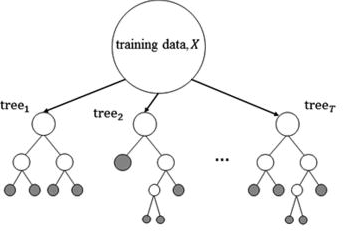
\includegraphics[width=3.4in]{tree_average.png}
\end{figure}
\end{frame}

\begin{frame}\frametitle{What is Bagging?}
\small 
\qu{Bagging} is a portmanteau of \qu{bootstrap} + \qu{aggregation} which are...\pause 

\begin{block}{Bootstrap (in our case, the \qu{nonparametric bootstrap})} \pause 
Sample the observations $1,\ldots,n$ with replacement. \pause You get only about 2/3 of the unique $n$ observations since you double and triple up.\\~\\ \pause 

What it means in this context is that each of the $T$ trees are built with a bootstrap sample. \pause Each tree itself is a \qu{weak learner} but many slightly different trees together is strong since they reduce variance from overfitting (beyond scope of course).\pause
\end{block}

\begin{block}{Aggregation}
What we said before: \qu{aggregate} the $\yhat$'s from the $T$ trees together via average (regression) or majority vote (classification). \pause 
\end{block}

Bagging beats single trees... but once we bag, no interpretability anymore! Complete black box due to that function $\hat{f}$ being so complicated!!

\end{frame}

\begin{frame}\frametitle{Random Forests (RF)}

To reduce variance between the trees, we have to bust up the correlation structure between each tree. \pause The last piece of the puzzle Breiman cracked in 2001: each tree only sees a sample of the features. \pause Each tree only sees $p^* < p$. \\~\\ \pause

This was we do this, the predictive accuracy then beats bagging (no one uses just bagging anymore). \emph{These many trees taken together as a unit do not overfit!!!}
	
\begin{block}{Random Forests (RF) Algorithm} \pause
\begin{itemize}
\item Build many overfit trees
\item In each tree use a sample with replacement of the rows
\item In each tree use a sample of the availabe features \pause
\end{itemize}
\end{block}


\end{frame}


\begin{frame}\frametitle{RF \qu{Tuning Parameters}}


\begin{itemize}
\item Number of trees --- we want a lot to reduce variance (default is 500 in R)
\item Number of splitting features for a individual tree --- we want less than $p$ to decorrelate (default $p/3$ for regression and $\sqrt{p}$ for classification)
\item Number of observations in smallest split node --- we want to overfit (default is 5 in regression, 1 in classification)
\end{itemize}

The amazing thing is ... \pause the defaults work so well, you hardly ever need to change them!! \emph{RF in my opinion is the best predictive model out-of-the-box.}
\end{frame}


\begin{frame}\frametitle{Tuning RF --- Nested Resampling}

Remember this from last class? Here's where it's used... But I do \inred{not recommend} doing this!

\begin{figure}
\centering
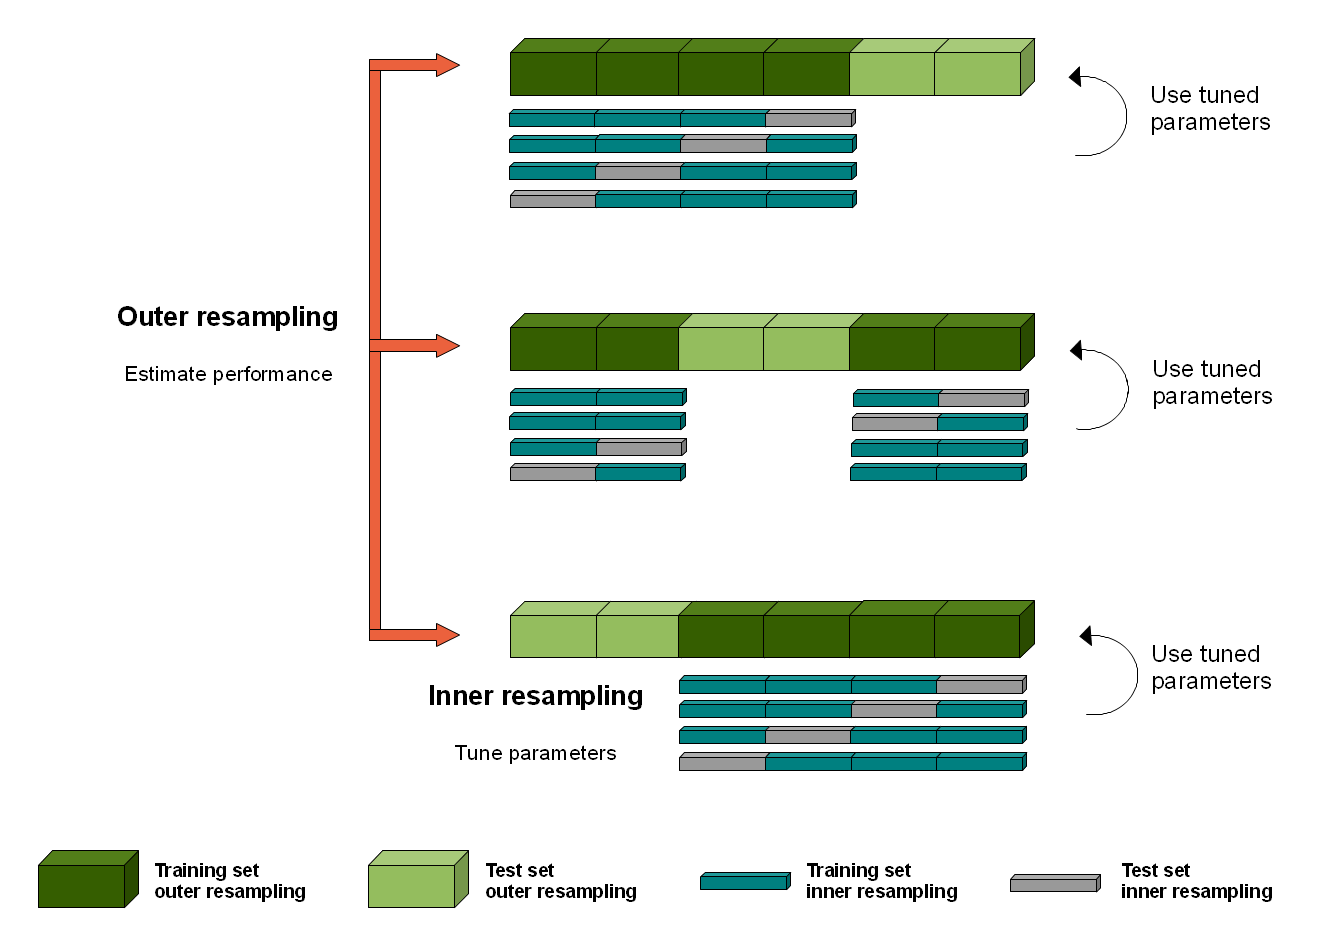
\includegraphics[width=3.36in]{nested_resampling_for_tuning.png}
\end{figure}

(from \href{https://mlr-org.github.io/mlr-tutorial/devel/html/nested_resampling/index.html}{MLR's tutorial website}).
\end{frame}

\begin{frame}\frametitle{A Nice Perk in RF --- OOB Estimation}

So RF doesn't overfit, but how do we assess this? \pause we can use oos validation (plain or with $K$-fold CV), but we don't have to! Why? \pause Each tree was built with a bootstrap sample. This means $\approx$ 2/3 of the $n$ observations were used to build the tree and therefore $\approx$ 1/3 of the $n$ observations were not! Aren't those $\approx$ 1/3 that were not oos? \pause YES! \pause These $\approx$ 1/3 are called \qu{out of bag} (OOB). Over the many $T$ trees, all $n$ observations went out of bag many times giving us many trees to get oos average for each observation. \\~\\ \pause


\tiny
(Note: this strategy can be used for any modeling procedure as an alternative to $K$-fold CV and MLR in R gives you this option... I'm still not sure why $K$-fold CV is the default). \\~\\ \pause
	
\end{frame}


\begin{frame}\frametitle{When does RF win / lose?}
\pause
\begin{itemize}
\item Signal is high, noise is low (no one wins when signal is low, noise is high). I've seen the linear model and RF performing about equal in high noise cases. \pause
\item When there truly are lots of interactions among the predictors and curvilinear relationships with the response. \pause
\item When there are not \qu{too many} features. $p > n$ is a problem for everyone. RF can find what it believes to be a nice predictor, but it's really fake and only idiosyncratically related to the response.
\end{itemize}

Demo time...

\end{frame}

\begin{frame}\frametitle{JMP 1/4}

\begin{figure}
\centering
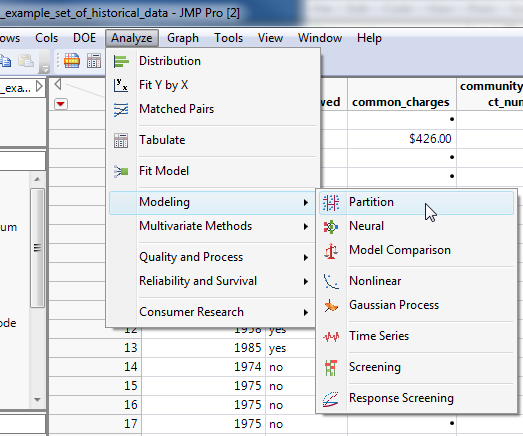
\includegraphics[width=3.5in]{jmp01.png}
\end{figure}
\end{frame}


\begin{frame}\frametitle{JMP 2/4}

\begin{figure}
\centering
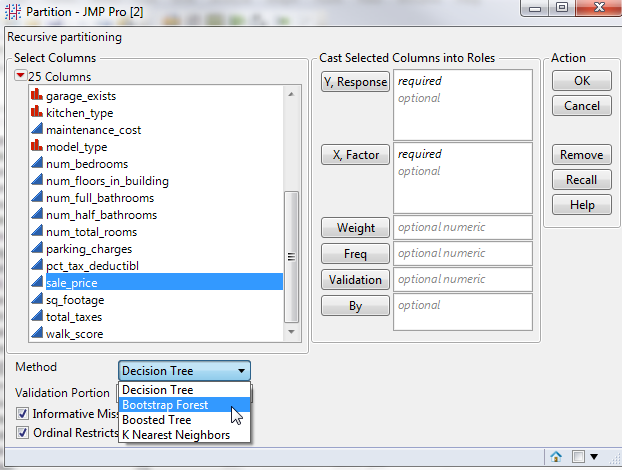
\includegraphics[width=3.5in]{jmp02.png}
\end{figure}
	
\end{frame}

\begin{frame}\frametitle{JMP 3/4}

\begin{figure}
\centering
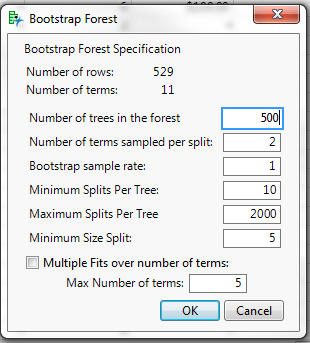
\includegraphics[width=3.0in]{jmp03.png}
\end{figure}
	
\end{frame}


\begin{frame}\frametitle{JMP 4/4}

\begin{figure}
\centering
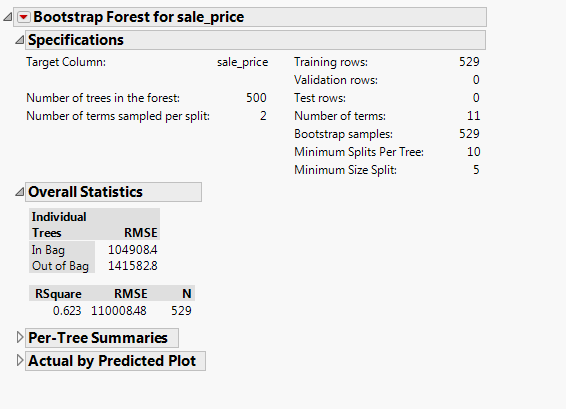
\includegraphics[width=3.1in]{jmp04.png}
\end{figure}
You don't need to do oos validation on Random Forests as the \qu{out of bag} is as good as oos.
\end{frame}

\begin{frame}[fragile]\frametitle{R 1/2}

\begin{verbatim}
#load the data
X = read.csv(
 "stat_422_722_project_example_set_of_historical_data.csv")
#recode sale_price as a number
X$sale_price = as.numeric(gsub('[$,]','',
  as.character(X$sale_price)))
#install and load up the RF package
install.packages("randomForest")
library(randomForest)
#run the RF
rf_mod = randomForest(sale_price ~ 
	coop_condo + num_bedrooms + 
	num_full_bathrooms + walk_score, X)
rf_mod #print out its output
\end{verbatim}


\end{frame}

\begin{frame}\frametitle{R 2/2}

\begin{figure}
\centering
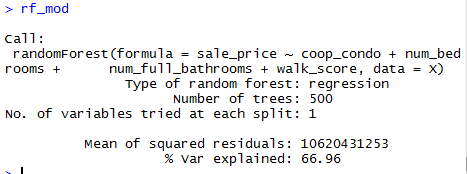
\includegraphics[width=4.1in]{R01.png}
\end{figure}

\end{frame}

\section{Course Conclusion!}

\begin{frame}\frametitle{We Made It! Now a Summary and Review...}
\small
A quick review of the topics (and the topics that will not be covered on the final next week).\\~\\

\textbf{Lecture 1}

\begin{itemize}
\item Definitions of prediction, model, response, feature / predictor, observation \pause
\item Mathematizing English into measurements so we can create models \pause
\item We talked about mathematical models, statistical models and the conditional expectation function $f$. \pause
\item Types of data: continuous, categorical. We talked about binning to convert continuous $\rightarrow$ categorical. \pause
\item Raw data represenations and deep learning, featurization to $p$ measurable features \pause
\item Meehl's work on basic statistical models beating humans \pause
\item Data collection: sampling and measurement to create a data frame
\end{itemize}

\end{frame}

\begin{frame}\frametitle{Review...}

\begin{itemize}
\item Good machine learning (sampling and featurization) vs. bad machine learning (mindless data dumps of convenience)
\item Parametric vs non-parametric worldview when modeling
\item Definition of parameters
\item Definition of parameter estimates (model fitting)
\item Residuals and loss functions (\emph{SSE}$^\star$, SAE)
\item Measures of fit: $R^2$, $SSE$, $RMSE$ and their interpretations and their equivalence
\item Empirical rule $\yhat \pm RMSE$
\end{itemize}
	
\end{frame}

\begin{frame}\frametitle{Review...}

\textbf{Lecture 2}

\begin{itemize}
\item Graphical causal models with bubbles and arrows
\item Definition of noise in statistical models
\item Probabilistic Causation
\item Three sources of noise (1) Irreducible Error (2) Model Misspecification due to a parametric assumption (3) Model Estimation Error
\item The reasonable assumption of $\errorrv$ distributed normally
\item The four OLS assumptions and what this buys you
\item What a likelihood is and what a log-likelihood is
\item What maximum likelihood estimation is
\item What the likelihood ratio is and when to reject (big values that exceed critical $\chisq{}$ values)
\end{itemize}
	
\end{frame}

\begin{frame}\frametitle{Review...}

\begin{itemize}
\item OLS regression: Omnibus / global $F$-tests
\item OLS regression: Partial $F$-test
\item OLS regression: $t$-test
\item OLS regression: how to predict ($\yhat$ calculations)
\item Proper interpretation of $\betahat_j$
\item Causation and correlation
\item Lurking / confounding predictors
\item Spurious (or coincidental) correlations
\item Natural observation vs. manipulated measurements
\item Randomized experiments can reveal additive causal effects
\item Why \qu{science is impossible}
\item Why collinearity may invalidate $\betahat_j$ interpretation
\item Why correlations are still useful
\end{itemize}
	
\end{frame}

\begin{frame}\frametitle{Review...}

\begin{itemize}
\item Data dredging
\item Multiple testing correction with Bonferroni (hedges against dredging)
\item Generalizability of models
\end{itemize}
	
\textbf{Lecture 3}

\begin{itemize}
\item Extrapolation (a violation of generalizability)
\item How different modeling strategies extrapolate differently
\item Optimal design in linear models (over sample predictors' extreme values)
\item Optimal design in highly non-parametric models (more towards even spacing throughout predictors' ranges)
\item Odds, logistic link function and its sigmoidal shape, logit function (log odds)
\item Fitting $\betahat_j$'s in logistic regression
\end{itemize}

\end{frame}

\begin{frame}\frametitle{Review...}
%\small
\begin{itemize}
\item How to draw inference in logistic regression (likelihood ratio test)
\item How to predict conditional probabilities $\phat$'s in logistic regression
\item How to use classification rules based on a threshold $\phat_0$
\item Confusion Matrices, FN, FP, TP, TN, sensitivity, specificity, FNR, FPR, FDR, FOR
\item ROC Curve, ROC table and AUC metric
\end{itemize}
	
\textbf{Lecture 4}

\begin{itemize}
\item Asymmetric costs in classification, weighted misclassification error, minimizing this metric to find best $p_0$
\item Survival Model --- the response and why it's censored
\item Interpreting $\betahat_j$ in an exponential survival model
\item How to draw inference in survival regression (likelihood ratio test)
\item Predictions in survival models

\end{itemize}
\end{frame}

\begin{frame}\frametitle{Review...}

\begin{itemize}
\item Testing linearity for one covariate in linear regression
\item Interpreting quadratic effects
\item Interpreting interaction effects
\item Overfitting and optimizing for the idiosyncratic $\errorrv$ terms
\item In-sample vs. oos metrics of fit (complexity-fit tradeoff curves)
\item Single training-test splits for oos validation
\item The test set as a lockbox that can be opened once and only once
\item Tradeoffs for training-test split sizes
\end{itemize}
	
\textbf{Lecture 5}

\begin{itemize}
\item $K$-fold cross validation (CV)
\item Advantage of doing $K$-fold CV
\item Using three splits to perform model selection
\end{itemize}
	
\end{frame}

\begin{frame}\frametitle{Review...}

\begin{itemize}
\item Missing data: selection models vs. pattern mixture models
\item Mechanisms: MCAR, MAR, NMAR
\item Why listwise deletion is nothing to write home about
\item Imputation under missingness due to each of the three mechanisms
\item Creating missingness features (the $\m$'s)
\item Forward stepwise regression using $t$-test, AICc and $R^2$ in a oos set
\end{itemize}
	
\textbf{Lecture 6}

\begin{itemize}
\item Binning --- advantages and disadvantages
\item Better bins through greedy splitting (decision trees)
\item Leaf assignment in decision trees
\item Pruning / stopping the growth of decision trees
\item Advantages and disadvantages of decision trees
\end{itemize}
	
\end{frame}

\begin{frame}\frametitle{Review...}

\begin{itemize}
\item Model averaging over multiple trees
\item Bagging (bootstrap and aggregation)
\item Sampling predictors
\item The 3 ideas above together = random forests (RF)
\item OOB estimates as oos estimates
\item When RF performs well and when it does not
\end{itemize}
	
\end{frame}

\end{document} %%%%%%%%%%%%%%%%%%%%%%%%%%%%%%%%%
